\chapter{Hardware}\label{ch:hardware}
This chapter will give an overview of the hardware used for implementing a Kalman filter for the purpose of tracking a high altitude balloon.
It will also include answers to the SSEQ (Standard Sensor Exercise Questions) for the sensors used in the project.


\section{MCU}\label{sec:mcu}
The microcontroller used in this project is the STM32F446RE. The STM32F446RE is a 32-bit ARM Cortex-M4 microcontroller with a maximum CPU frequency of 180 MHz.
The microcontroller has 512 KB of flash memory and 128 KB of RAM.
The microcontroller has a variety of peripherals, including SPI, I2C, UART, and CAN.
This particular microcontroller was chosen because it is the microcontroller used in the student satlab organization, where the project is intended to be used.
The microcontroller can be seen in Figure~\ref{fig:stm32f446re}.
\begin{figure}[H]
    \centering
    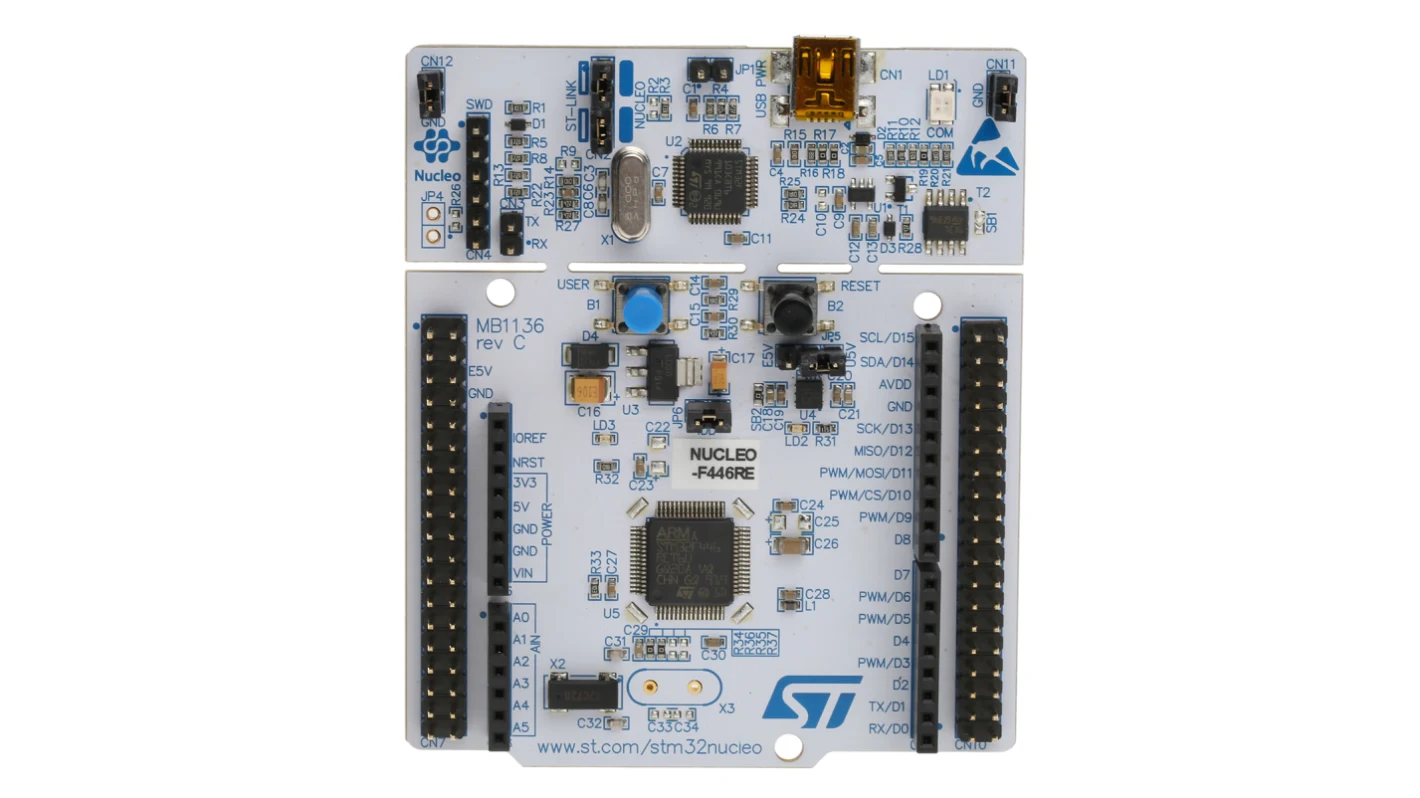
\includegraphics[width=0.8\textwidth]{chapters/02Harware/figures/stm32}
    \caption{The STM32F446RE microcontroller.}
    \label{fig:stm32f446re}
\end{figure}


\section{Barometer}\label{sec:barometer}
The barometer used in this project is the MS5611.
The MS5611 is a high-resolution pressure sensor. The purpose of the barometer is to measure the pressure, so an altitude can be calculated.
The MS5611 can measure pressure from 10 mbar to 1200 mbar, with a resolution of up to 0.012 mbar. %TODO: indsæt kilde
Since the expected maximum altitude of the balloon is around 15 km, the MS5611 is a suitable choice for this project.

\subsection{SSEQ for the MS5611}
\begin{enumerate}
    \item What is measured?
    \begin{enumerate}[(a)]
        \item Physical property/phenomenon measured?

        The physical property measured is the change in resistance of a material due to it being streched or compressed.
        This material is called a strain gauge.
        It is placed on a diaphragm, which moves when the pressure changes.
        The train gauge is connected to a Wheatstone bridge, which converts the change in resistance to a voltage.



        \item What are the units (physical phenomenon, output from sensor, desired signal)?

        The physical phenomenon is the change in resistance of the strain gauge, and therefore the unit of the physical phenomenon is Ohm.
        The output from the sensor is an ADC reading which represents as a voltage.
        The desired signal is the pressure in mbar, which can be calculated from the voltage using the datasheet of the sensor.

    \end{enumerate}

    \item Measuring
    \begin{enumerate}[(a)]
        \item What are the sampling frequency and resolution?

        Depending on the Oversampling Ratio, the conversion time can be between 0.5 ms and 8.22 ms.
        Which converts to 2000 Hz and 122 Hz respectively.
        At the highest resolution, the resolution is 0.012 mbar, and at the lowest resolution, the resolution is 0.065 mbar.


        \item Are measurements linear with the measured property?

        No they are not linear, since the resistance of the strain gauge both depends on the strain and the temperature.
        The sensor therefore also includes a temperature sensor, which can be used to compensate for the temperature dependency of the strain gauge.



        \item What is the conversion from raw measurements to proper measurements?

        Using the calibration data on the PROM of the sensor, the raw measurements can be converted to pressure in mbar.

        First the difference between the raw temperature and the reference temperature is calculated.
        Then the temperature is calculated using the reference temperature and the temperature sensitivity.

        The offset at the reference temperature is calculated using pressure offset and the temperature coefficient of the offset.

        Then the sensitivity at the actual temperature is calculated using the pressure sensitivity and the temperature coefficient of the pressure sensitivity. %TODO: måske indsætte alle de her ligninger.

        The temperature compensated pressure is then calculated using the formula:
        \begin{equation}
            P = D1 \cdot SENS - OFF
        \end{equation}
        Where $D1$ is the digital pressure value measured by the sensor, $SENS$ is the sensitivity at the actual temperature, and $OFF$ is the offset at the actual temperature.

        From this pressure, the altitude can be calculated using the Equation~\ref{eq:pressure2altitude}.
        \begin{equation}
            h = -\frac{log(\frac{P_m}{P_0}) \cdot T_0 \cdot R_0}{(M \cdot G_0)}
            \label{eq:pressure2altitude}
        \end{equation}
        Where $P_m$ is the measured pressure, $P_0$ is the pressure at sea level, $T_0$ is the temperature at sea level, $R_0$ is the universal gas constant, $M$ is the molar mass of the air, and $G_0$ is the acceleration due to gravity.

    \end{enumerate}
    \item Noise
    \begin{enumerate}[(a)]
        \item What type of noise to expect, and how noise depends on use and environment?
        Then noise in the barometer can be caused by the temperature of the sensor.
        Thermal noise is the noise from the thermal motion of the electrons in the sensor.
        This noise is proportional to the temperature of the sensor.
    \end{enumerate}
\end{enumerate}


\section{GNSS module}\label{sec:gnss-module}
The GNSS module used in this project is the u-blox NEO-6M.
This module can recieve signals from GPS, GLONASS, Galileo, and BeiDou satellites.
This module was chosen because it is the GNSS module used in the student satlab organization, where the project is intended to be used.

\subsection{SSEQ for the NEO-6M}
\begin{enumerate}
    \item What is measured?
    \begin{enumerate}[(a)]
        \item Physical property/phenomenon measured?
        The physical phenomenon measured is the time it takes for a signal to travel from a satellite to the receiver.
        This is done to multiple satellites, and the position of the receiver can be calculated using trilateration.

        \item Measuring principle or sensor operating principle?

        The reciever works by knowing the position of the satellites in the constellation, and the time it takes for the signal to travel from the satellite to the receiver.
        For each satellite, the receiver can calculate a sphere with the radius of the time it took for the signal to travel from the satellite to the receiver.
        The intersection of these spheres is the position of the receiver.
        The receiver needs to know the position of at least 4 satellites to get a fix, 3 for the position, and 1 for the time.


        \item What are the units (physical phenomenon, output from sensor, desired signal)?

        \textbf{The physical phenomenon:}
        The physical phenomenon is the time it takes for a signal to travel from a satellite to the receiver in seconds.

        \textbf{Output from the sensor:}
        The out from the sensor is follows the NMEA 183 standard.
        The data is transmitted in ASCII format, and includes information about the satellites in view, the position of the receiver, and the time of the measurement.
        In the NMEA 183 standard, there exists different sentence-types.
        Some include information about the position of the receiver, some include information about the signal to the constellation.
        The interesting sentences for this project are the GGA, RMC, and GLL sentences, since they include the position of the receiver.
        The units of the output include the position of the receiver in degrees, minutes, and seconds, the speed of the receiver in knots, and the course of the receiver in degrees.
        Furthermore, it also includes the SNR (Signal to Noise Ratio) of the signal from the satellites in dB.


        \textbf{Desired signal:}
        The desired signal is the position of the receiver, and the speed and course of the receiver.
        These can be found in the GGA and RMC sentences.
    \end{enumerate}
    \item Measuring
    \begin{enumerate}[(a)]
        \item What are the sampling frequency and resolution?
        The maximum navigation update rate is 5 Hz. %TODO: indsæt kilde. datasheet
        However, the time it takes to get a fix can be up to 27 seconds, depending on the environment and whether the module is coming from a cold start, warm start, or hot start.
        This is caused by the module needing to get the almanac and ephemeris data from the satellites.

        \item What is the conversion from raw measurements to proper measurements?
        The raw measurements are given in time in seconds, for the time it takes for a signal to travel from a satellite to the receiver.
        Assuming the speed of light is constant, the distance can be calculated by multiplying the time with the speed of light.

    \end{enumerate}
    \item Noise
    \begin{enumerate}[(a)]
        \item What type of noise to expect, and how noise depends on use and environment?
        The noise in the GNSS module can be caused by the signal being reflected off buildings, trees, or other objects thus taking longer to reach the receiver.

        Placing the GNSS module in an open area with a clear view of the sky can help reduce the noise.


        \item For determining noise, how and for how long should we sample?
        Determining the noise floor can be done by placing the GNSS module in an open area with a clear view of the sky, and then taking measurements over a long period of time.

    \end{enumerate}
    \item Testing
    \begin{enumerate}[(a)]
        \item What can we do to get different measurements (covering at least some of the sensor range)? Be creative!

        Since it is not feasible to actually put the sensor in a HAB, a way to get different measurements, at least in the latitudinal and longitudinal direction, is to move the sensor, for example by driving around with it ontop of a car.

        Getting different measurements in the altitude direction is more difficult, but could be done by moving the sensor up and down using a crane, ladder or a tall building.
    \end{enumerate}
\end{enumerate}






